\documentclass{report}

\input{~/dev/latex/template/preamble.tex}
\input{~/dev/latex/template/macros.tex}

\title{\Huge{}}
\author{\huge{Nathan Warner}}
\date{\huge{}}
\pagestyle{fancy}
\fancyhf{}
\lhead{Warner \thepage}
\rhead{}
% \lhead{\leftmark}
\cfoot{\thepage}
%\setborder
% \usepackage[default]{sourcecodepro}
% \usepackage[T1]{fontenc}

\begin{document}
    % \maketitle
    %     \begin{titlepage}
    %    \begin{center}
    %        \vspace*{1cm}
    % 
    %        \textbf{EAE 103} \\
    %        Assignment 5
    % 
    %        \vspace{0.5cm}
    %         
    %             
    %        \vspace{1.5cm}
    % 
    %        \textbf{Nathan Warner}
    % 
    %        \vfill
    %             
    %             
    %        \vspace{0.8cm}
    %      
    %        \includegraphics[width=0.4\textwidth]{}
    %             
    %        Computer Science \\
    %        Northern Illinois University\\
    %        September 25, 2023 \\
    %        United States\\
    %        
    %             
    %    \end{center}
    % \end{titlepage}
    % \tableofcontents
    \bigbreak \noindent 
    1.) In the first discussion board some of you expressed interest in topics not covered in this
class. Some of these are more suited for an astronomy (or astrophysics) class. Choose a topic of
interest to you not covered in the class (such as quasars, pulsars, neutron stars, galaxies,
quasars, cosmic rays, etc.), read about it in the textbook or from other credible sources, and
write a 30-50 word describing this feature and why you are interested in it.
    \bigbreak \noindent 
    \pf{Answer}{
        One topic that I find interesting that I would like to discuss is: \textbf{Neutron Stars:} These are incredibly dense remnants of supernova explosions. A teaspoon of neutron star material would weigh about a billion tons on Earth. I'm fascinated by the extreme conditions on these stars and how they challenge our understanding of physics.
    }

    \bigbreak \noindent 
    2.a)  Find an image of a Kuiper belt object, other than Pluto, and describe it
    \bigbreak \noindent 
    \pf{Answer}{
        \textbf{Ceres Images:} These images depict a celestial body that somewhat resemble our moon. Ceres is a rocky body that is covered in craters.
    }

    \bigbreak \noindent 
    2.b) ) Find an image of the cantaloupe terrain on Triton. Download the image and include it with this exercise. 
    \bigbreak \noindent 
    \pf{Answer}{
        \bigbreak \noindent 
    \begin{center}
        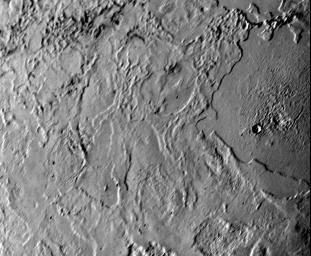
\includegraphics[scale=0.5]{./PIA02208.jpg}
    \end{center}
    }

    \bigbreak \noindent 
    2.c) What is the cantaloupe terrain made of, and how did it form? 
    \bigbreak \noindent 
    \pf{Answer}{
    The cantaloupe terrain, like much of Triton's surface, is largely made up of frozen water ice. One  idea of its formation is that the crust was subjected to extensional forces, causing it to stretch and crack in a specific pattern.
    }
    
    \bigbreak \noindent 
    2.d) Download and include an image from Uranus’ moon Ariel showing grooves and canyons
    \bigbreak \noindent 
    \pf{Answer}{
    \bigbreak \noindent 
    \begin{center}
        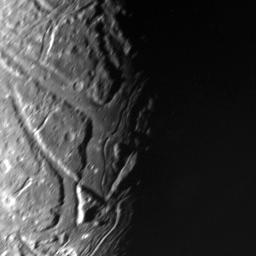
\includegraphics[scale=0.5]{./PIA01356.jpg}
    \end{center}
    }

    \bigbreak \noindent 
    2.e) What could be causing these grooves and canyons? 
    \bigbreak \noindent 
    \pf{Answer}{
     Much of Ariel's surface is cut by extensive fault valleys, some of which are over 10 km wide. These fault valleys are likely to have formed as a result of extensional forces stretching Ariel's crust. As the crust stretched, portions of it dropped down, forming the valleys.
    }

    \bigbreak \noindent 
    3.a) In the notes I show an image of a cryo-volcano on Pluto (Wright-Mons). (a) What types of
    materials erupt from Plutonian cryo-volcanoes? 
    \begin{itemize}
        \item Water ice
        \item Nitrogen ice
        \item Ammonia
        \item Methane and Carbon Monoxide
    \end{itemize}

    \bigbreak \noindent 
    3.b) What does this tell us about Pluto’s interior? 
    \begin{itemize}
        \item Possible subsurface ocean or warm layer.
        \item Internal heat source, potentially from radioactive decay.
        \item Dynamic geological history.
        \item Presence of ammonia suggests "antifreeze" properties, aiding in maintaining a subsurface ocean.
    \end{itemize}

    \bigbreak \noindent 
    4.) List two methods used by astronomers to identify extra-solar planets (exoplanets). 
    \bigbreak \noindent 
    \pf{Answer}{
        \bigbreak \noindent 
    \begin{itemize}
        \item \textbf{Transit Method:} Astronomers monitor the brightness of a star over time. If a planet crosses in front of its star (from our point of view), it causes a temporary drop in the star's brightness. This is called a transit.
        \item \textbf{Radial Velocity or Doppler Method:} Astronomers measure the star's spectrum to detect a wobble in its motion caused by the gravitational pull of an orbiting planet.
    \end{itemize}
    }

    \bigbreak \noindent 
    5.) Write the Drake Equation (which estimates the number of intelligent civilizations in our
    galaxy capable of communication) and define each of the terms.
    \bigbreak \noindent 
    \begin{align*}
        N_{c} = N_{*} \cdot f_{p} \cdot n_{HZ} \cdot f_{L} \cdot f_{I} \cdot f_{S}
    .\end{align*}
    Where:
    \begin{itemize}
        \item $N_{*}$  = number of stars in our galaxy
        \item $f_{P}$  = fraction of stars with planets
        \item $n_{HZ}$  = average number of planets in each planetary system in the Goldilocks (habitable) zone
        \item $f_{L}$  = fraction of planets on which life begins
        \item $f_{I}$  = fraction of planets with life that have intelligent life
        \item $f_{S}$  = fraction of a star’s life during which a civilization is communicative
    \end{itemize}









\end{document}
